\documentclass[12pt]{article}
\usepackage{array,booktabs}
\usepackage{graphicx} % Required for inserting images
\usepackage{setspace}
\usepackage[margin=2.5cm]{geometry} % margins
\usepackage[parfill]{parskip}
\usepackage{enumitem}
\usepackage{amsfonts,latexsym,amsthm,amssymb,amsmath,amscd,euscript}

%Chemistry Packages
\usepackage{chemfig}
\usepackage{mhchem}
\usepackage{chemformula}
\usepackage{siunitx}
\usepackage{pgfplots}
\sisetup{group-digits=false}
\usepackage{cancel}

\pgfplotsset{compat=1.18}

\setlength{\parindent}{0pt}
\AtBeginDocument{\setstretch{1.125}}

\title{Yeast Lab}
\author{Anthony Yu}
\date{October 2024}

\begin{document}

%Some new commands
\newcommand{\problem}[1]{\subsection*{Problem {#1}}}
\newenvironment{enumAlph}{\begin{enumerate}[label=(\alph*)]}{\end{enumerate}}

\makeatletter
\newcommand{\skipitems}[1]{%
\addtocounter{\@enumctr}{#1}%
}
\makeatother

\newcommand{\chunit}[3]{\qty{#1}{{#2}\,\ce{#3}}}
\newcommand{\chuniteval}[3]{\qty[evaluate-expression]{#1}{{#2}\,\ce{#3}}}

\newtheorem{definition}{Definition}


\maketitle

\begin{center}
    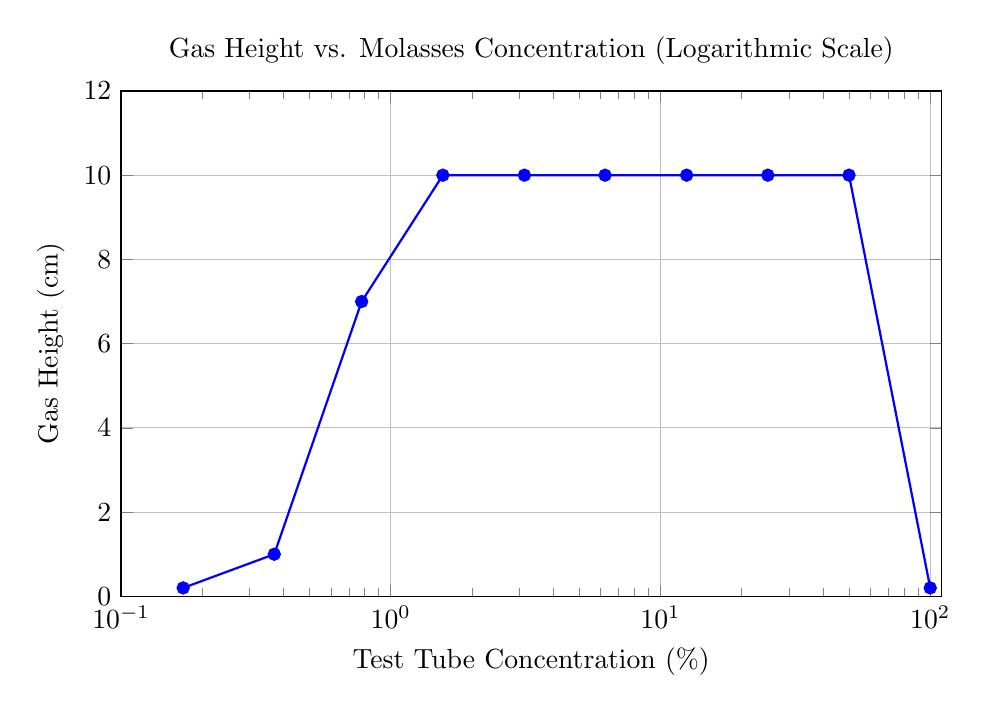
\begin{tikzpicture}
        \begin{axis}[
            width=12cm, % Width of the plot
            height=8cm, % Height of the plot
            xlabel={Test Tube Concentration (\%)},
            ylabel={Gas Height (cm)},
            ymin=0, ymax=12,
            xmode=log, % Set the x-axis to a logarithmic scale
            xmin=0.1, xmax=110,
            grid=major,
            title={Gas Height vs. Molasses Concentration (Logarithmic Scale)}
        ]
        \addplot[
            mark=*,
            blue,
            thick
        ] coordinates {
            (100, 0.2)
            (50, 10)
            (25, 10)
            (12.5, 10)
            (6.23, 10)
            (3.13, 10)
            (1.56, 10)
            (0.78, 7.0)
            (0.37, 1.0)
            (0.17, 0.2)
        };
        \end{axis}
    \end{tikzpicture}
    \end{center}

\end{document}